% -*- TeX-engine: xetex; -*-
% Compile with XeLaTeX

%%%%%%%%%%%%%%%%%%%%%%%
% To do before class
%%%%%%%%%%%%%%%%%%%%%%%

% Send the Logistics/Week0Annoucnement (the night before).
% Send an email reminding students to bring a charged computer (the night before).

%%%%%%%%%%%%%%%%%%%%%%%
% Option 1: Slides: (comment for handouts)   %
%%%%%%%%%%%%%%%%%%%%%%%

\documentclass[slidestop,compress,mathserif,12pt,t,professionalfonts,xcolor=table]{beamer}

% solution stuff
\newcommand{\solnMult}[1]{
\only<1>{#1}
\only<2->{\red{\textbf{#1}}}
}
\newcommand{\soln}[1]{\textit{#1}}

%%%%%%%%%%%%%%%%%%%%%%%%%%%%%%%
% Option 2: Handouts, without solutions (post before class)    %
%%%%%%%%%%%%%%%%%%%%%%%%%%%%%%%

% \documentclass[11pt,containsverbatim,handout,xcolor=xelatex,dvipsnames,table]{beamer}

% % handout layout
% \usepackage{pgfpages}
% \pgfpagesuselayout{4 on 1}[letterpaper,landscape,border shrink=5mm]

% % solution stuff
% \newcommand{\solnMult}[1]{#1}
% \newcommand{\soln}[1]{}

% % % This breaks things for me for some reason.
% % tell pgfpages how to set page sizes in XeLaTeX
% %\renewcommand\pgfsetupphysicalpagesizes{%
% %   \pdfpagewidth\pgfphysicalwidth\pdfpageheight\pgfphysicalheight%
% %}

%%%%%%%%%%%%%%%%%%%%%%%%%%%%%%%%%%%%
% Option 3: Handouts, with solutions (may post after class if need be)    %
%%%%%%%%%%%%%%%%%%%%%%%%%%%%%%%%%%%%

% \documentclass[11pt,containsverbatim,handout,xcolor=xelatex,dvipsnames,table]{beamer}

% % handout layout
% \usepackage{pgfpages}
% \pgfpagesuselayout{4 on 1}[letterpaper,landscape,border shrink=5mm]

% % solution stuff
% \newcommand{\solnMult}[1]{\red{\textbf{#1}}}
% \newcommand{\soln}[1]{\textit{#1}}

% % % This breaks things for me for some reason.
% % % tell pgfpages how to set page sizes in XeLaTeX
% % \renewcommand\pgfsetupphysicalpagesizes{%
% %    \pdfpagewidth\pgfphysicalwidth\pdfpageheight\pgfphysicalheight%
% % }

%%%%%%%%%%%%%%%%%%%%%%%%%%%%%%%
% Option 4: Notes Only
%%%%%%%%%%%%%%%%%%%%%%%%%%%%%%%

% % See http://tex.stackexchange.com/questions/114219/add-notes-to-latex-beamer
% \documentclass[10pt,containsverbatim,xcolor=xelatex,dvipsnames,table,notes=only]{beamer}

% % handout layout
% % \usepackage{pgfpages}
% % \pgfpagesuselayout{1 on 1}[letterpaper, landscape, border shrink=5mm]

% % solution stuff
% \newcommand{\solnMult}[1]{#1}
% \newcommand{\soln}[1]{}

% % % Having a problem with this.
% % tell pgfpages how to set page sizes in XeLaTeX
% % \renewcommand\pgfsetupphysicalpagesizes{%
% %   \pdfpagewidth\pgfphysicalwidth\pdfpageheight\pgfphysicalheight%
% %}

%%%%%%%%%%
% Load style file, defaults  %
%%%%%%%%%%

%%%%%%%%%%%%%%%%
% Themes
%%%%%%%%%%%%%%%%

% See http://deic.uab.es/~iblanes/beamer_gallery/ for mor options

% Style theme
\usetheme{Pittsburgh}

% Color theme
\usecolortheme{seahorse}

% Font theme
%\usepackage[T1]{fontenc}
%\usepackage[scaled=0.92]{helvet}

%\usepackage[no-math]{fontspec}
%\setsansfont{TeX Gyre Heros}
% "TeX Gyre Heros can be used as a replacement for Helvetica"
% In Unix, unzip the following into ~/.fonts
% In Mac, unzip it, double-click the .otf files, and install using "FontBook"
%   http://www.gust.org.pl/projects/e-foundry/tex-gyre/heros/qhv2.004otf.zip

\usepackage{fontspec}

%%%%%%%%%%%%%%%%
% Packages
%%%%%%%%%%%%%%%%

\usepackage{geometry}
\usepackage{graphicx}
\usepackage{amssymb}
\usepackage{epstopdf}
\usepackage{amsmath}  	% this permits text in eqnarray among other benefits
\usepackage{url}		% produces hyperlinks
\usepackage[english]{babel}
\usepackage[latin1]{inputenc}
\usepackage{colortbl}	% allows for color usage in tables
\usepackage{multirow}	% allows for rows that span multiple rows in tables
\usepackage{color}		% this package has a variety of color options
\usepackage{colortbl}
\usepackage{pgf}
\usepackage{calc}
\usepackage{ulem}
\usepackage{multicol}
\usepackage{textcomp}
\usepackage{txfonts}
\usepackage{listings}
\usepackage{tikz}
\usepackage{fancyvrb}

%%%%%%%%%%%%%%%%
% Remove navigation symbols
%%%%%%%%%%%%%%%%

\beamertemplatenavigationsymbolsempty
\hypersetup{pdfpagemode=UseNone} % don't show bookmarks on initial view

%%%%%%%%%%%%%%%%
% User defined colors
%%%%%%%%%%%%%%%%

% Pantone 2015 Spring colors
% http://iwork3.us/2014/09/16/pantone-2015-spring-fashion-report/
% update each semester or year

\xdefinecolor{custom_blue}{rgb}{0, 0.70, 0.79} % scuba blue
\xdefinecolor{custom_darkBlue}{rgb}{0.11, 0.31, 0.54} % classic blue
\xdefinecolor{custom_orange}{rgb}{0.97, 0.57, 0.34} % tangerine
\xdefinecolor{custom_green}{rgb}{0.49, 0.81, 0.71} % lucite green
\xdefinecolor{custom_red}{rgb}{0.58, 0.32, 0.32} % marsala

\xdefinecolor{custom_lightGray}{rgb}{0.78, 0.80, 0.80} % glacier gray
\xdefinecolor{custom_darkGray}{rgb}{0.54, 0.52, 0.53} % titanium

%%%%%%%%%%%%%%%%
% Template colors
%%%%%%%%%%%%%%%%

\setbeamercolor*{palette primary}{fg=white,bg= custom_blue}
\setbeamercolor*{palette secondary}{fg=black,bg= custom_blue!80!black}
\setbeamercolor*{palette tertiary}{fg=white,bg= custom_blue!80!black!80}
\setbeamercolor*{palette quaternary}{fg=white,bg= custom_blue}

\setbeamercolor{structure}{fg= custom_blue}
\setbeamercolor{frametitle}{bg= custom_blue!90}
\setbeamertemplate{blocks}[shadow=false]
\setbeamersize{text margin left=2em,text margin right=2em}

%%%%%%%%%%%%%%%%
% Styling fonts, bullets, etc.
%%%%%%%%%%%%%%%%

% styling of itemize bullets
\setbeamercolor{item}{fg=custom_blue}
\setbeamertemplate{itemize item}{{{\small$\blacktriangleright$}}}
\setbeamercolor{subitem}{fg=custom_blue}
\setbeamertemplate{itemize subitem}{{\textendash}}
\setbeamerfont{itemize/enumerate subbody}{size=\footnotesize}
\setbeamerfont{itemize/enumerate subitem}{size=\footnotesize}

% styling of enumerate bullets
\setbeamertemplate{enumerate item}{\insertenumlabel.}
\setbeamerfont{enumerate item}{family={\fontspec{Helvetica Neue}}}
\setbeamerfont{enumerate subitem}{family={\fontspec{Helvetica Neue}}}
\setbeamerfont{enumerate subsubitem}{family={\fontspec{Helvetica Neue}}}

% make frame titles small to make room in the slide
\setbeamerfont{frametitle}{size=\small} 

% set Helvetica Neue font for frame and section titles
\setbeamerfont{frametitle}{family={\fontspec{Helvetica Neue}}}
\setbeamerfont{sectiontitle}{family={\fontspec{Helvetica Neue}}}
\setbeamerfont{section in toc}{family={\fontspec{Helvetica Neue}}}
\setbeamerfont{subsection in toc}{family={\fontspec{Helvetica Neue}}, size=\small}
\setbeamerfont{footline}{family={\fontspec{Helvetica Neue}}}
\setbeamerfont{subsection in toc}{family={\fontspec{Helvetica Neue}}}
\setbeamerfont{block title}{family={\fontspec{Helvetica Neue}}}

%%%%%%%%%%%%%%%%
% Color text commands
%%%%%%%%%%%%%%%%

%orange
\newcommand{\orange}[1]{\textit{\textcolor{custom_orange}{#1}}}

% green
\newcommand{\green}[1]{\textit{\textcolor{custom_green}{#1}}}

% red
\newcommand{\red}[1]{\textit{\textcolor{custom_red}{#1}}}

% dark gray
\newcommand{\darkgray}[1]{\textit{\textcolor{custom_darkGray}{#1}}}

% light gray
\newcommand{\lightgray}[1]{\textit{\textcolor{custom_lightGray}{#1}}}


%%%%%%%%%%%%%%%%
% Custom commands
%%%%%%%%%%%%%%%%

% cancel
\newcommand{\cancel}[1]{%
    \tikz[baseline=(tocancel.base)]{
        \node[inner sep=0pt,outer sep=0pt] (tocancel) {#1};
        \draw[red, line width=0.5mm] (tocancel.south west) -- (tocancel.north east);
    }%
}

% degree
\newcommand{\degree}{\ensuremath{^\circ}}

% cite
\newcommand{\ct}[1]{
\vfill
{\tiny #1}}

% Note
\newcommand{\Note}[1]{
\rule{2.5cm}{0.25pt} \\ \textit{\footnotesize{\textcolor{custom_red}{Note:} \textcolor{custom_darkGray}{#1}}}}

% Remember
\newcommand{\Remember}[1]{\textit{\scriptsize{\textcolor{custom_red}{Remember:} #1}}}

% links: webURL, webLink
\newcommand{\webURL}[1]{\urlstyle{same}{\textit{\textcolor{custom_blue}{\url{#1}}}}}
\newcommand{\webLink}[2]{\href{#1}{\textcolor{custom_blue}{{#2}}}}

% mail
\newcommand{\mail}[1]{\href{mailto:#1}{\textit{\textcolor{custom_blue}{#1}}}}

% highlighting: hl, hlGr, mathhl
\newcommand{\hl}[1]{\textit{\textcolor{custom_blue}{#1}}}
\newcommand{\hlGr}[1]{\textit{\textcolor{custom_green}{#1}}}
\newcommand{\mathhl}[1]{\textcolor{custom_blue}{\ensuremath{#1}}}

% example
\newcommand{\ex}[1]{\textcolor{blue}{{{\small (#1)}}}}

% two col: two columns
\newenvironment{twocol}[4]{
\begin{columns}[c]
\column{#1\textwidth}
#3
\column{#2\textwidth}
#4
\end{columns}
}

% slot (for probability calculations)
\newenvironment{slot}[2]{
\begin{array}{c} 
\underline{#1} \\ 
#2
\end{array}
}

% pr: left and right parentheses
\newcommand{\pr}[1]{
\left( #1 \right)
}

%%%%%%%%%%%%%%%%
% Custom blocks
%%%%%%%%%%%%%%%%

% activity: less commonly used
\newcommand{\activity}[2]{
\setbeamertemplate{itemize item}{{{\small\textcolor{custom_orange}{$\blacktriangleright$}}}}
\setbeamercolor{block title}{fg=white, bg=custom_orange}
\setbeamerfont{block title}{size=\small}
\setbeamercolor{block body}{fg=black, bg=custom_orange!20!white!80}
\setbeamerfont{block body}{size=\small}
\begin{block}{Activity: #1}
#2
\end{block}
}

% app: application exercise
\newcommand{\app}[2]{
\setbeamercolor{block title}{fg=white,bg=custom_green}
\setbeamercolor{block body}{fg=black,bg=custom_green!20!white!80}
\begin{block}{{\small Application exercise: #1}}
#2
\end{block}
}

% disc: discussion question
\newcommand{\disc}[1]{
\setbeamercolor{block body}{bg=custom_blue!25!white!80, fg=custom_blue!55!black!95}
\begin{block}{\vspace*{-3ex}}
#1
\end{block}
}

% clicker: clicker question
\newcommand{\clicker}[1]{
\setbeamercolor{block title}{bg=custom_blue!80!white!50,fg=custom_blue!30!black!90}
\setbeamercolor{block body}{bg=custom_blue!20!white!80,fg=custom_blue!30!black!90}
\begin{block}{\vspace*{-0.2ex}{\footnotesize Clicker question}\vspace*{-0.2ex}}
#1
\end{block}
}

% formula
\newcommand{\formula}[2]{
\setbeamercolor{block title}{bg=custom_blue!40!white!60,fg=custom_blue!55!black!95}
\begin{block}{{\small#1}}
#2
\end{block}
}

% code
\newcommand{\code}[1]{
\newfontfamily{\monaco}{Monaco}
{\monaco {\footnotesize \textcolor{custom_darkBlue}{#1}}}
}

% output
\renewcommand{\output}[1]{
{\monaco {\footnotesize \textcolor{custom_darkGray}{#1}}}
}

%%%%%%%%%%%%%%%%
% Change margin
%%%%%%%%%%%%%%%%

\newenvironment{changemargin}[2]{%
\begin{list}{}{%
\setlength{\topsep}{0pt}%
\setlength{\leftmargin}{#1}%
\setlength{\rightmargin}{#2}%
\setlength{\listparindent}{\parindent}%
\setlength{\itemindent}{\parindent}%
\setlength{\parsep}{\parskip}%
}%
\item}{\end{list}}

%%%%%%%%%%%%%%%%
% Footnote
%%%%%%%%%%%%%%%%

\long\def\symbolfootnote[#1]#2{\begingroup%
\def\thefootnote{\fnsymbol{footnote}}\footnote[#1]{#2}\endgroup}

%%%%%%%%%%%%%%%%
% Graphics
%%%%%%%%%%%%%%%%

\DeclareGraphicsRule{.tif}{png}{.png}{`convert #1 `dirname #1`/`basename #1 .tif`.png}

%%%%%%%%%%%%%%%%
% Slide number
%%%%%%%%%%%%%%%%

\setbeamertemplate{footline}{%
    \raisebox{5pt}{\makebox[\paperwidth]{\hfill\makebox[20pt]{\color{gray}
          \scriptsize\insertframenumber}}}\hspace*{5pt}}

          
%%%%%%%%%%%%%%%%
% Remove page numbers
%%%%%%%%%%%%%%%%

\newcommand{\removepagenumbers}{% 
  \setbeamertemplate{footline}{}
}

%%%%%%%%%%%%%%%%
% TOC slides
%%%%%%%%%%%%%%%%

% TRY TO CHANGE THE ENUMERATE SYMBOLS HERE FROM CIRCLES TO PLAIN NUMBERS

\AtBeginSection[] 
{ 
  \addtocounter{framenumber}{-1} 
  % 
  {\removepagenumbers 
    \begin{frame}<beamer> 
    \tableofcontents[currentsection] 
  \end{frame} 
  } 
}
% You cannot use numbers when defining variables.  Hence the use of letters, A, B, C, etc.

% Personal Info
\newcommand{\FirstName}{Mine}
\newcommand{\LastName}{\c{C}etinkaya-Rundel}
\newcommand{\OfficeHours}{MTWR 3-4pm.}
\newcommand{\OfficeHoursLocation}{Old Chem 213}

% Electronic Info
\newcommand{\PersonalSite}{http://stat.duke.edu/~mc301}
\newcommand{\CourseSite}{http://bitly.com/sta101sp15}
\newcommand{\Email}{mine@stat.duke.edu}

% TAs
\newcommand{\TAA}{Anthony Weishampel}
\newcommand{\TAB}{Fiamma Li}
\newcommand{\TAC}{Jialiang Mao}
\newcommand{\TAD}{Phillip Lee}

% Exam Dates
\newcommand{\ExamADate}{Wed, Feb 18}
\newcommand{\ExamBDate}{Wed, Mar 25}
\newcommand{\FinalDate}{Sat, May 2 (2-5pm)}

% Due Dates
\newcommand{\ClickerRegistrationDD}{Mon, Jan 26}
\newcommand{\GettingToKnowYouDD}{Friday, Jan 9, 11:59pm}
\newcommand{\ProblemSetADD}{Wed., 1/15}


% ALT ALT
% % You cannot use numbers when defining variables.  Hence the use of letters, A, B, C, etc.

% Personal Info
\renewcommand{\FirstName}{Jesse}
\renewcommand{\LastName}{Windle}
\renewcommand{\OfficeHours}{Tue, Thu 3:00pm-4:30pm}

% Electronic Info
\renewcommand{\PersonalSite}{http://stat.duke.edu/~jbw44/}
\renewcommand{\CourseSite}{http://bitly.com/windle2}
\renewcommand{\Email}{jbw44@stat.duke.edu}

% TAs
\renewcommand{\TAA}{David Clancy}
\renewcommand{\TAB}{Xinyi (Chris) Li}
\renewcommand{\TAC}{Tori Hall}
\renewcommand{\TAD}{Radhika Anand}

% Exam Dates
\renewcommand{\ExamADate}{Thu, Feb 19}
\renewcommand{\ExamBDate}{Thu, Mar 26}
\renewcommand{\FinalDate}{Mon, Apr 27 (9-Noon)}

% Due Dates
\renewcommand{\ClickerRegistrationDD}{Thu, Jan 15}
\renewcommand{\GettingToKnowYouDD}{Friday, Jan 9, 11:59pm}

%%%%%%%%%%%
% Cover slide info    %
%%%%%%%%%%%

\title{Unit 3: Foundations for inference}
\subtitle{1. Variability in estimates and CLT}
\author{Sta 101 - Spring 2015}
\date{February 9, 2015}
% ALT ALT 
% \date{February 10, 2015}
\institute{Duke University, Department of Statistical Science}

%%%%%%%%%%%
% Begin document   %
%%%%%%%%%%%

\begin{document}

%%%%%%%%%%%%%%%%%%%%%%%%%%%%%%%%%%%%

% Title Page

\begin{frame}[plain]

\titlepage
\vfill
{\scriptsize \webLink{\PersonalSite}{Dr. \LastName{}} \hfill Slides posted at  \webLink{\CourseSite}{\CourseSite}}
\addtocounter{framenumber}{-1} 

\end{frame}

%%%%%%%%%%%%%%%%%%%%%%%%%%%%%%%%%%%%

\section{Housekeeping}

%%%%%%%%%%%%%%%%%%%%%%%%%%%%%%%%%%%%

\begin{frame}
\frametitle{Announcements}

\begin{itemize}

\item MT Review: Monday, Feb 16, 7-8pm at Old Chemistry 116

% ALT ALT

% \item Exam 1: Thu, Feb. 19.

% \item Rest of videos for Unit 3: I recommend you finish them by Thursday.

% \item Lab 4 due Wed.

% \item PS 5 due Thu.

\end{itemize}

%---Note---%
\note{

Readiness Assessment 3

Question 1: NOTATION.  (c) What is suggestion that may be
skewed?  Natural boundary and std deviation.

Question 2: What is the definition of the standard deviation?  Standard error?

Standard error refers to standard deviation of a sampling distribution.

Question 3: Need to add ``sample'' to standard deviation.

Ask what is wrong with (c).

Question 4: Go through why each statement is wrong.

Question 10: Go through each answer.

Grade example for confidence level.
Weather example for confidence level.

}

\end{frame}

%%%%%%%%%%%%%%%%%%%%%%%%%%%%%%%%%%%%

\section{Main ideas}

%%%%%%%%%%%%%%%%%%%%%%%%%%%%%%%%%%%%

\subsection{Sample statistics vary from sample to sample}
\label{mi1}

%%%%%%%%%%%%%%%%%%%%%%%%%%%%%%%%%%%%

\begin{frame}
\frametitle{Sample statistics vary from sample to sample}

\begin{itemize}

\item We are often interested in \hl{population parameters}.

\item Since complete populations are difficult (or impossible) to collect data on, we use \hl{sample statistics} as \hl{point estimates} for the unknown population parameters of interest.

\item Sample statistics vary from sample to sample.

\item Quantifying how sample statistics vary provides a way to estimate the \hl{margin of error} associated with our point estimate.

\item But before we get to quantifying the variability among samples, let's try to understand how and why point estimates vary from sample to sample.

\end{itemize}

% ALT ALT
% \pause

\disc{Suppose we randomly sample 1,000 adults from each state in the US. Would you expect the sample means of their ages to be the same, somewhat different, or very different?}

%---Note---%
\note{

Pop parameter: what is the average GPA at Duke?

}

\end{frame}

%%%%%%%%%%%%%%%%%%%%%%%%%%%%%%%%%%%

\begin{frame}
\frametitle{}

\disc{We would like to estimate the average number of drinks it takes students to get drunk. 
\begin{itemize}
\item We will assume that our population is comprised of 146 students.
\item Assume also that we don't have the resources to collect data from all 146, so we will take a sample of size $n = 10$. 
\end{itemize}
If we randomly select observations from this data set, which values are most likely to be selected, which are least likely?}

\begin{center}
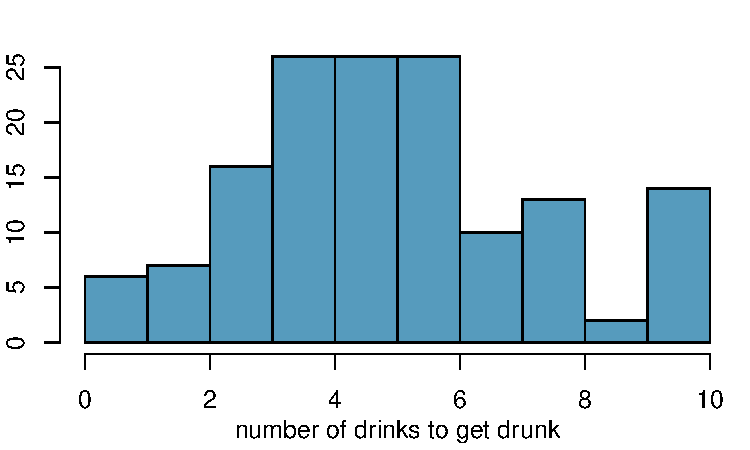
\includegraphics[width=0.6\textwidth]{figures/no_drinks_drunk/hist_no_drinks_drunk_pop} 
\end{center}

%---Note---%
\note{

}

\end{frame}

%%%%%%%%%%%%%%%%%%%%%%%%%%%%%%%%%%%

\begin{frame}[fragile]
\frametitle{}

\begin{itemize}

\item Sample, with replacement, ten student IDs:
{\footnotesize
\begin{Verbatim}[frame=single, formatcom=\color{blue}]
> sample(1:146, size = 10, replace = TRUE)
\end{Verbatim}
}
\pause
{\footnotesize
\begin{Verbatim}[frame=single, formatcom=\color{gray}]
[1]  59 121  88  46  58  72  82  81   5  10
\end{Verbatim}
}
\pause

\item Find the students with these IDs:

\begin{center}
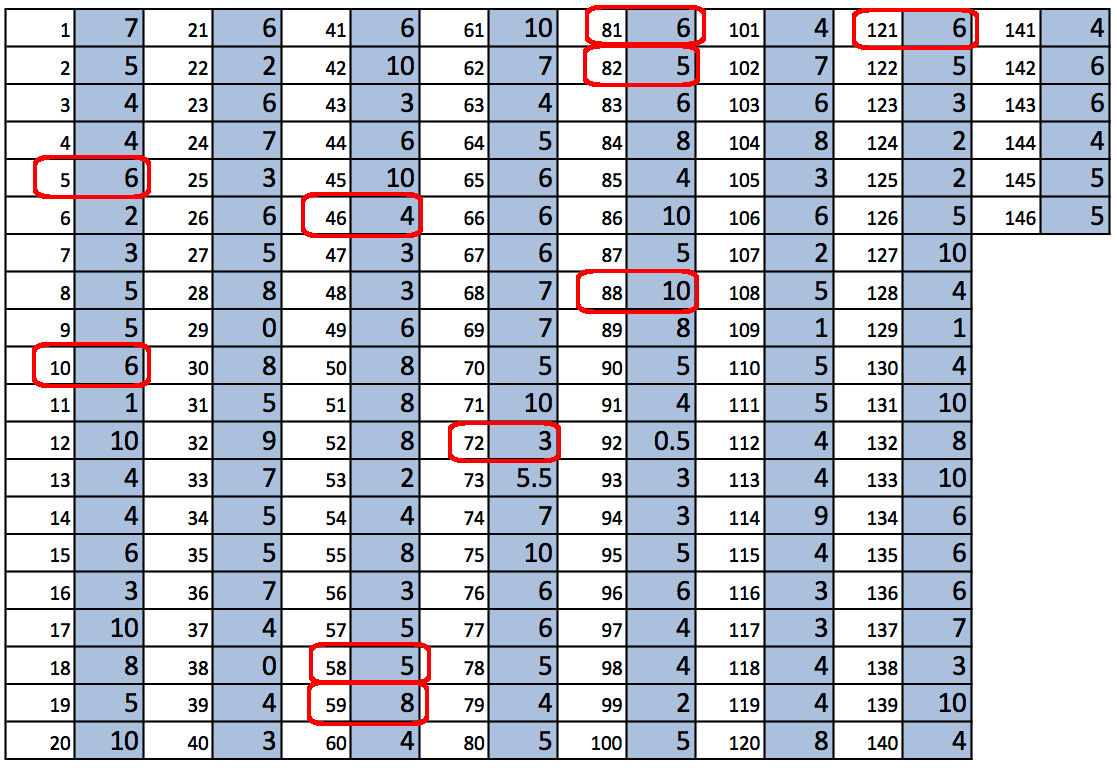
\includegraphics[width=0.65\textwidth]{figures/no_drinks_drunk/no_drinks_drunk_mysample}
\end{center}

\pause

\item Calculate the sample mean: $(8+6+10+4+5+3+5+6+6+6) / 10 = 5.9$

\end{itemize}

%---Note---%
\note{

}

\end{frame}

%%%%%%%%%%%%%%%%%%%%%%%%%%%%%%%%%%%%

\begin{frame}[fragile]
\frametitle{}

\activity{Creating a sampling distribution}{Repeat this in teams, and report your sample mean.}
\begin{enumerate}

\item Sample, with replacement, ten student IDs:
{\footnotesize
\begin{Verbatim}[frame=single, formatcom=\color{blue}]
> sample(1:146, size = 10, replace = TRUE)
\end{Verbatim}
}

\item Find the students with these IDs:

\begin{center}
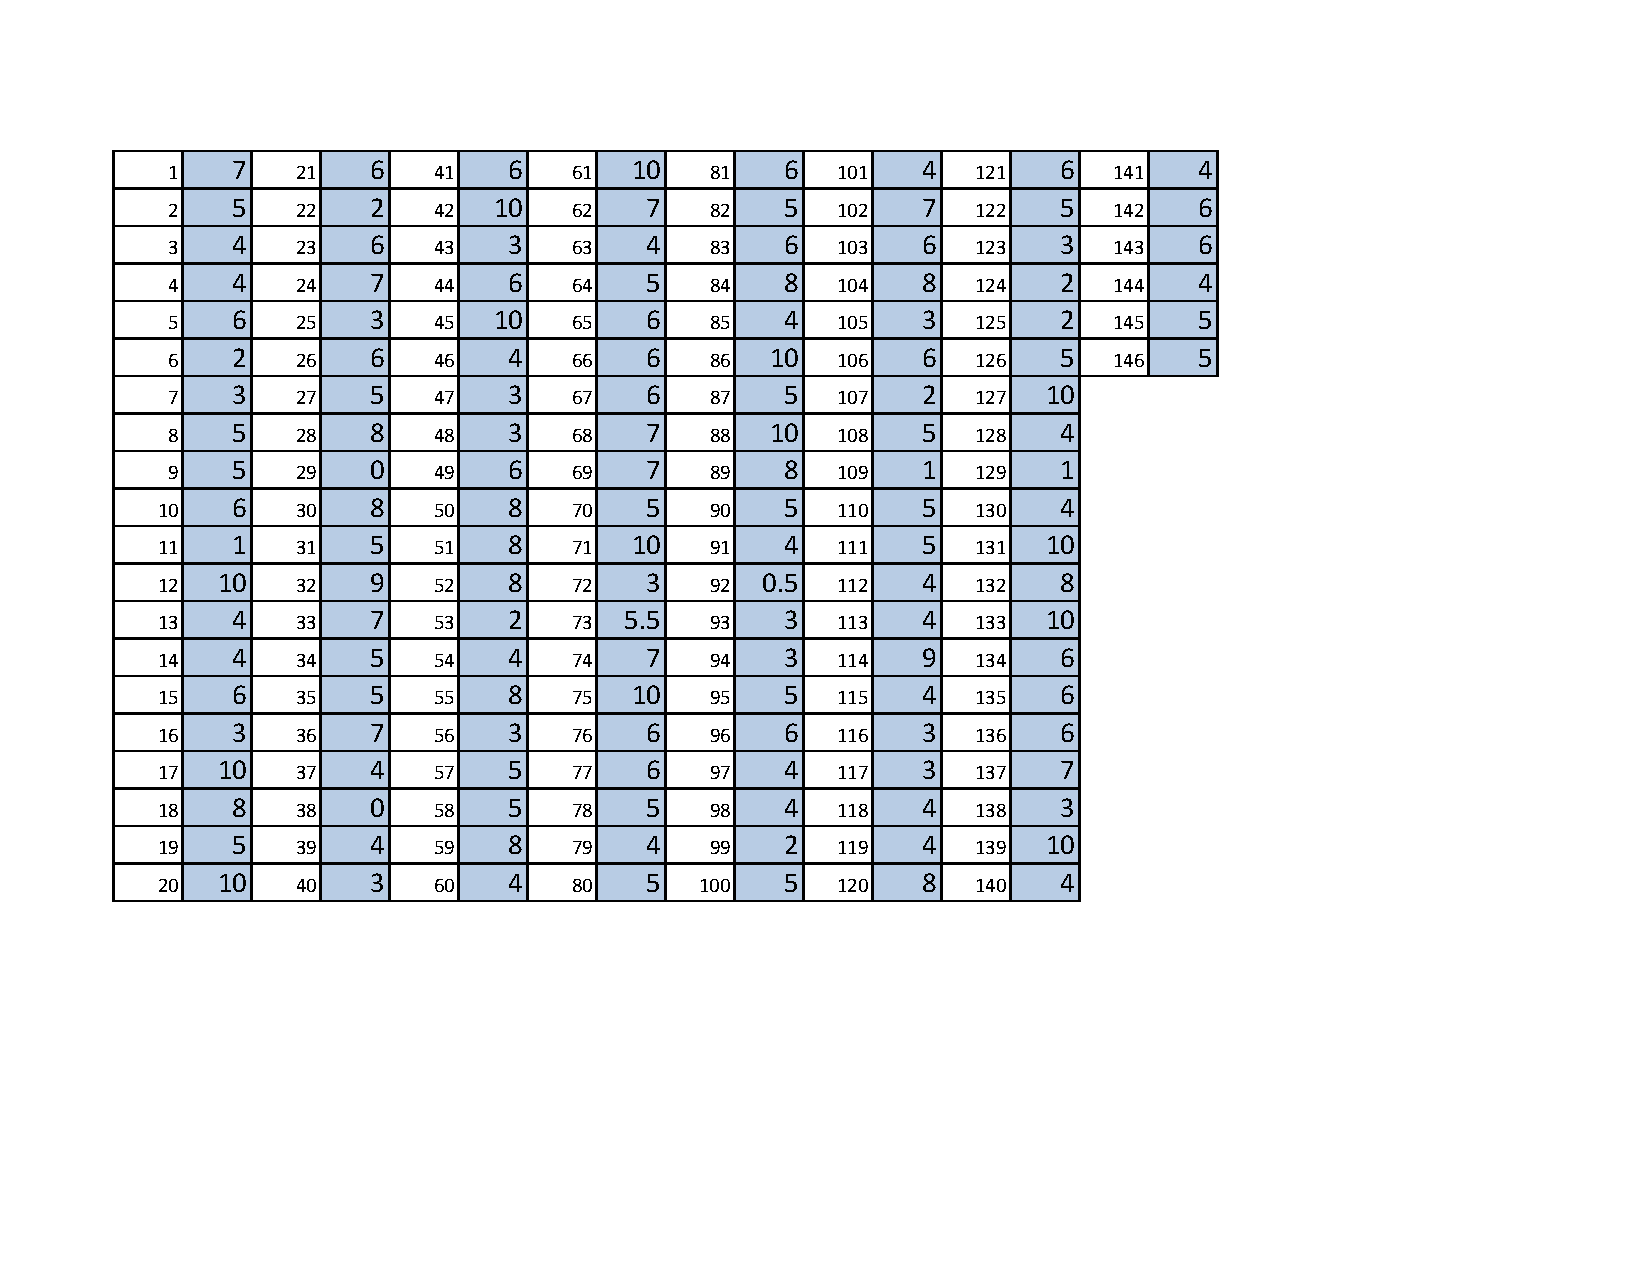
\includegraphics[width=0.6\textwidth]{figures/no_drinks_drunk/no_drinks_drunk_clean}
\end{center}

\item Calculate the sample mean, round it to 2 decimal places, and submit it using your clicker. Submit once per sample!

\end{enumerate}

%---Note---%
\note{

Take a sample from population.

Do activity: use clicker and report answer to two decimal places.

(5 minutes?)

}

\end{frame}

%%%%%%%%%%%%%%%%%%%%%%%%%%%%%%%%%%%

\begin{frame}[fragile]
\frametitle{Sampling distribution}

What you just constructed is called a \hl{sampling distribution}.

$\:$ \\
\disc{What is the shape and center of this distribution. Based on this distribution what do you think is the true population average?}

$\:$ \\
\soln{\only<2>{
5.39
}}

\end{frame}


%%%%%%%%%%%%%%%%%%%%%%%%%%%%%%%%%%%%

\begin{frame}[fragile]
\frametitle{Average number of Duke games attended}

Next let's look at the population data for the number of Duke basketball games attended:

\begin{center}
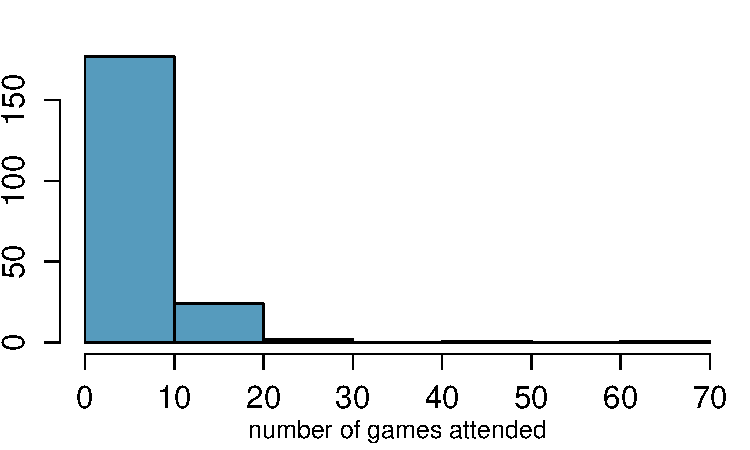
\includegraphics[width=0.8\textwidth]{figures/duke_games/hist_duke_games_pop}
\end{center}



\end{frame}

%%%%%%%%%%%%%%%%%%%%%%%%%%%%%%%%%%%%

\begin{frame}[fragile]
\frametitle{Average number of Duke games attended (cont.)}

Sampling distribution, n = 10:

\twocol{0.6}{0.4}{
\begin{center}
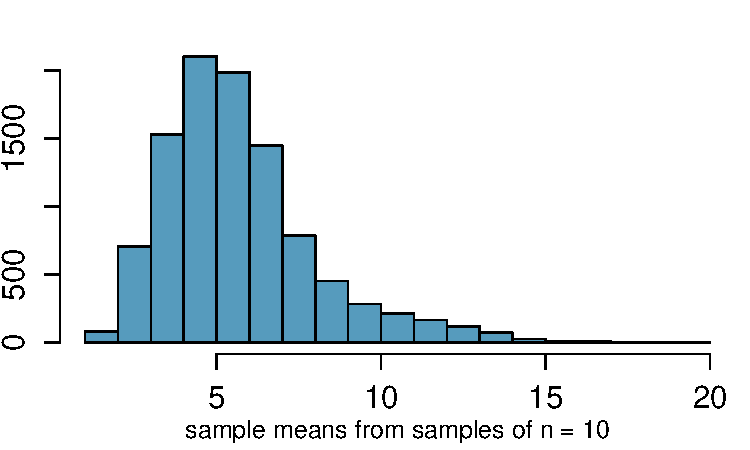
\includegraphics[width=\textwidth]{figures/duke_games/hist_duke_games_sampling10}
\end{center}
}
{
\disc{What does each observation in this distribution represent?}
\soln{\only<2->{Sample mean, $\bar{x}$, of samples of size $n = 10$.}}
\disc{Is the variability of the sampling distribution smaller or larger than the variability of the population distribution?}
\soln{\only<3->{Smaller, sample means will vary less than individual observations.}}
}

%---Note---%
\note{

What measure of spread is useful?  Range.

}

\end{frame}


%%%%%%%%%%%%%%%%%%%%%%%%%%%%%%%%%%%%

\begin{frame}[fragile]
\frametitle{Average number of Duke games attended (cont.)}

Sampling distribution, n = 30:

\twocol{0.6}{0.4}{
\begin{center}
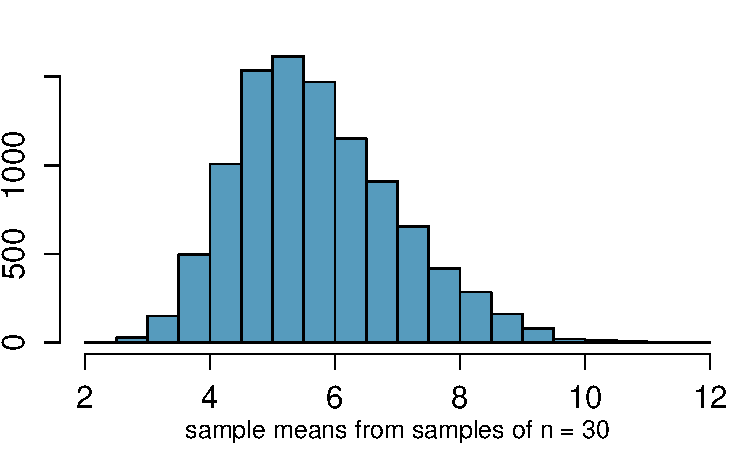
\includegraphics[width=\textwidth]{figures/duke_games/hist_duke_games_sampling30}
\end{center}
}
{
\disc{How did the shape, center, and spread of the sampling distribution change going from $n = 10$ to $n = 30$?}
\soln{\only<2->{Shape is more symmetric, center is about the same, spread is smaller.}}
}

%---Note---%
\note{



}

\end{frame}


%%%%%%%%%%%%%%%%%%%%%%%%%%%%%%%%%%%%

\begin{frame}[fragile]
\frametitle{Average number of Duke games attended (cont.)}

Sampling distribution, n = 70:

\begin{center}
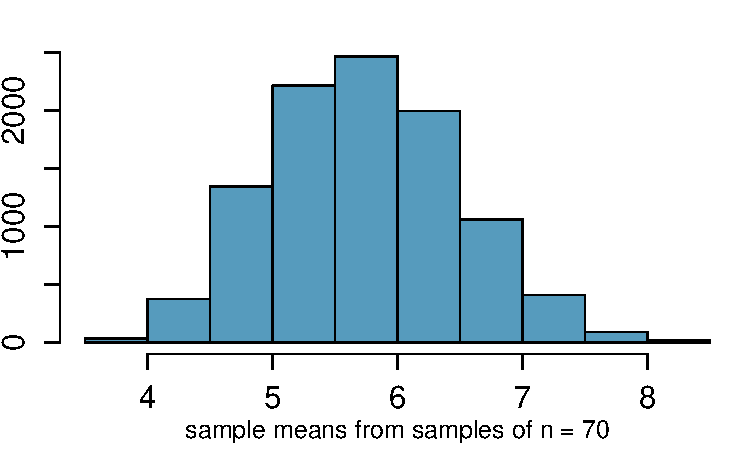
\includegraphics[width=0.6\textwidth]{figures/duke_games/hist_duke_games_sampling70}
\end{center}

\end{frame}


%%%%%%%%%%%%%%%%%%%%%%%%%%%%%%%%%%%%

\begin{frame}[fragile]
\frametitle{Average number of Duke games attended (cont.)}

\clicker{The mean of the sampling distribution is 5.75, and the standard deviation of the sampling distribution (also called the \hl{standard error}) is 0.75. Which of the following is the most reasonable guess for the 95\% confidence interval for the true average number of Duke games attended by students?}

\begin{enumerate}[(a)]
\item $5.75 \pm 0.75$
\item \solnMult{$5.75 \pm 2 \times 0.75$} \soln{\only<2>{\red{$\rightarrow (4.25,7.25)$}}}
\item $5.75 \pm 3 \times 0.75$
\item cannot tell from the information given
\end{enumerate}

%---Note---%
\note{

Could elimintate this?

Make sure to go back to multiple choice.

}

\end{frame}

%%%%%%%%%%%%%%%%%%%%%%%%%%%%%%%%%%%%

\subsection{CLT describes the shape, center, and spread of sampling distributions}
\label{mi2}

%%%%%%%%%%%%%%%%%%%%%%%%%%%%%%%%%%%%

\begin{frame}
\frametitle{2. CLT describes the shape, center, and spread of sampling distributions}


The distribution of the sample means is well approximated by a normal model:
\[ \bar{x} \sim N \pr{ mean = \mu, SE = \frac{\sigma}{\sqrt{n}} } \]
If $\sigma$ is unknown, use $s$.
% ALT ALT
% \emph{Under the right conditions}, the distribution of the sample means is well
% approximated by a normal distribution:
% \[ \bar{x} \sim N \pr{ mean = \mu, SE = \frac{\sigma}{\sqrt{n}} } \]
% A cheat: If $\sigma$ is unknown, use $s$.

\pause

\begin{itemize}

\item So it wasn't a coincidence that the sampling distributions we saw earlier were symmetric.

\item We won't go into the proving why $SE =  \frac{\sigma}{\sqrt{n}}$, but note that as $n$ increases $SE$ decreases. 

\item As the sample size increases we would expect samples to yield more consistent sample means, hence the variability among the sample means would be lower.

\end{itemize}
% ALT ALT
% \begin{itemize}

% \item As sample size increases, spread of sampling distribution decreases:
% \[
% SE = \frac{\sigma}{\sqrt{n}}.
% \]

% \end{itemize}

%---Note---%
\note{

Emphasize standard error is standard deviation of statistics.  And that it
depends on $n$.  So as you get more samples, your error should decrease.

}

\end{frame}

%%%%%%%%%%%%%%%%%%%%%%%%%%%%%%%%%%%%

\subsection{CLT only applies when independence and sample size/skew conditions are met}
\label{mi3}

%%%%%%%%%%%%%%%%%%%%%%%%%%%%%%%%%%%%

\begin{frame}
\frametitle{3. CLT only applies when independence and sample size/skew conditions are met}

\begin{enumerate}

\item \hlGr{Independence:} Sampled observations must be independent. \\

$\:$ \\
This is difficult to verify, but is more likely if
\begin{itemize}
\item random sampling/assignment is used, and,
\item if sampling without replacement, $n$ $<$ 10\% of the population.
\end{itemize}

\pause

\item \hlGr{Sample size/skew:} Either the population distribution is normal \\
or\\
$n > 30$ and the population distribution is not extremely skewed (the more skewed the distribution, the higher $n$ necessary for the CLT to apply).\\
$\:$ \\
This is also difficult to verify for the population, but we can check it using the sample data, and assume that the sample mirrors the population.
% ALT ALT
% \item \hlGr{Sample size/skew:} Either 

% \begin{enumerate}
% \item the population distribution is normal or

% \item $n > 30$ and the population dist.\ is not extremely skewed, or

% \item $n >> 30$ (approx.\ gets better as $n$ increases).
% \end{enumerate}

% This is also difficult to verify for the population, but we can check it using the sample data, and assume that the sample mirrors the population.

% END ALT

\end{enumerate}

%---Note---%
\note{

When can you use CLT?

6500 students at Duke.  Try to use that to motivate 10\% rule.

How sould you actually verify this?

}

\end{frame}

%%%%%%%%%%%%%%%%%%%%%%%%%%%%%%%%%%%%

\begin{frame}
\frametitle{3. CLT only applies when independence and sample size/skew conditions are met}

Amongst other things, the central limit theorem is useful for 
\begin{itemize}
\item constructing confidence intervals and
\item conducting hypothesis tests.
\end{itemize}

\end{frame}

%%%%%%%%%%%%%%%%%%%%%%%%%%%%%%%%%%%%

\begin{frame}
\frametitle{}

\clicker{Which of the below visualizations is \emph{not} appropriate for checking the shape of the distribution of the sample, and hence the population?}

\begin{enumerate}[(a)]
\item histogram
\item boxplot
\item normal probability plot
\item \solnMult{mosaicplot}
\end{enumerate}

%---Note---%
\note{

What do we use a mosaic plot for?  What type of data do we use a mosaic plot for?

}

\end{frame}

%%%%%%%%%%%%%%%%%%%%%%%%%%%%%%%%%%%%

\section{Summary}

%%%%%%%%%%%%%%%%%%%%%%%%%%%%%%%%%%%%

\begin{frame}
\frametitle{Summary of main ideas}

\vfill

\begin{enumerate}

\item \nameref{mi1}

\item \nameref{mi2}

\item \nameref{mi3}

\end{enumerate}

\vfill

\end{frame}

%%%%%%%%%%%%%%%%%%%%%%%%%%%%%%%%%%%

\section{Exercises [time permitting]}

%%%%%%%%%%%%%%%%%%%%%%%%%%%%%%%%%%%

\begin{frame}
\frametitle{}

\clicker{
{\footnotesize Four plots: Determine which plot (A, B, or C) is which. \\
(1) At top: distribution for a population ($\mu = 60, \sigma = 18$), \\
(2) a single random sample of 500 observations from this population, \\
(3) a distribution of 500 sample means from random samples with size 18,  \\
(4) a distribution of 500 sample means from random samples with size 81.}}

\twocol{0.4}{0.6}{
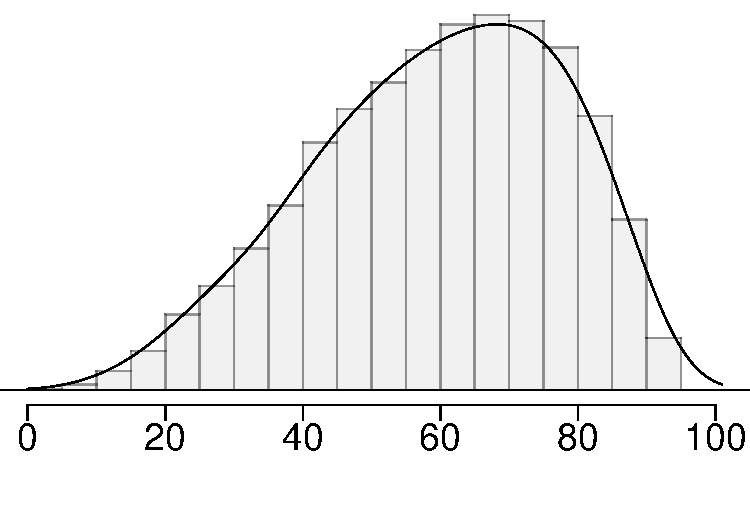
\includegraphics[width=\textwidth]{figures/cltSimLS/cltSimLS_pop}
}
{
\vspace{-0.5cm}
{\small
\begin{enumerate}[(a)]
\item (2) - B; (3) - A; (4) - C
\item (2) - A; (3) - B; (4) - C
\item (2) - C; (3) - A; (4) - D
\item \solnMult{(2) - B; (3) - C; (4) - A}
\end{enumerate}
}
}
\vspace{-0.25cm}
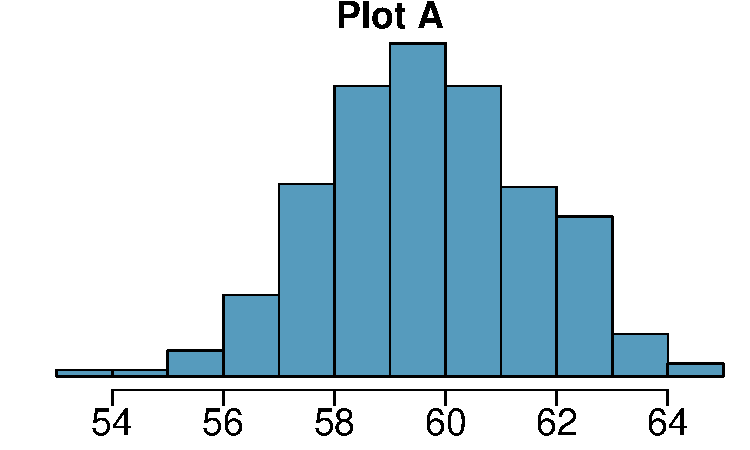
\includegraphics[width=0.32\textwidth]{figures/cltSimLS/cltSimLS_n81}
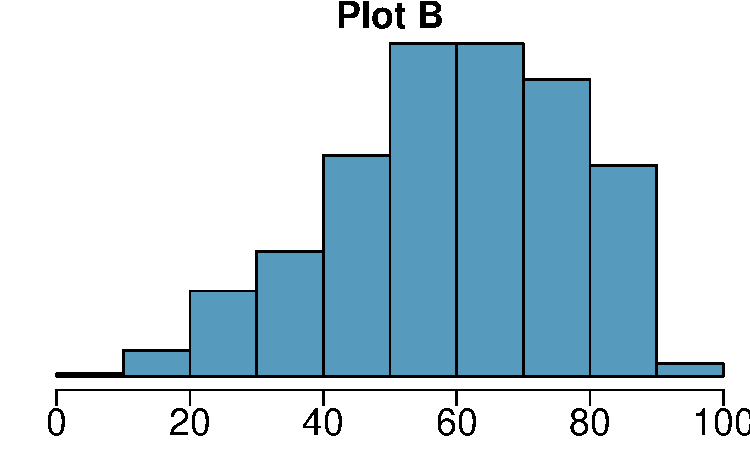
\includegraphics[width=0.32\textwidth]{figures/cltSimLS/cltSimLS_samp}
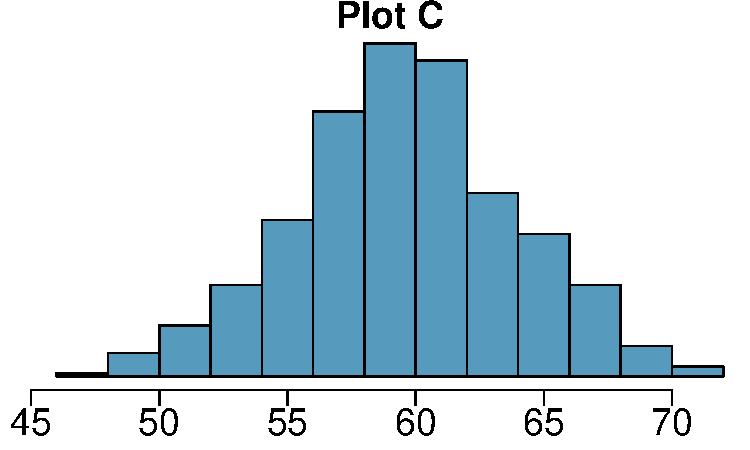
\includegraphics[width=0.32\textwidth]{figures/cltSimLS/cltSimLS_n18}

\end{frame}

%%%%%%%%%%%%%%%%%%%%%%%%%%%%%%%%%%%%

\begin{frame}

\disc{{\small A housing survey was conducted to determine the price of a typical home in Topanga, CA. The mean price of a house was roughly \$1.3 million with a standard deviation of \$300,000. There were no houses listed below \$600,000 but a few houses above \$3 million.}}

\disc{{\small Would you expect most houses in Topanga to cost more or less than \$1.3 million? Hint: What is most likely the shape of this distribution?}}

\pause

\soln{Since the distribution is probably right skewed, the median would be less than the mean, and a majority of observations would be lower than the mean.}


\end{frame}

%%%%%%%%%%%%%%%%%%%%%%%%%%%%%%%%%%%%

\begin{frame}

\disc{{\small A housing survey was conducted to determine the price of a typical home in Topanga, CA. The mean price of a house was roughly \$1.3 million with a standard deviation of \$300,000. There were no houses listed below \$600,000 but a few houses above \$3 million.}}

\clicker{Can we estimate the probability that a randomly chosen house in Topanga costs more than \$1.4 million using the normal distribution?}

\begin{enumerate}[(a)]
\item yes
\item \solnMult{no}
\end{enumerate}

\end{frame}

%%%%%%%%%%%%%%%%%%%%%%%%%%%%%%%%%%%

\begin{frame}

\disc{{\small A housing survey was conducted to determine the price of a typical home in Topanga, CA. The mean price of a house was roughly \$1.3 million with a standard deviation of \$300,000. There were no houses listed below \$600,000 but a few houses above \$3 million.}}

\clicker{Can we estimate the probability that the mean of 60 randomly chosen houses in Topanga is more than \$1.4 million?}

\begin{enumerate}[(a)]
\item \solnMult{yes}
\item no
\end{enumerate}

\end{frame}

%%%%%%%%%%%%%%%%%%%%%%%%%%%%%%%%%%%%

\begin{frame}

\disc{{\small A housing survey was conducted to determine the price of a typical home in Topanga, CA. The mean price of a house was roughly \$1.3 million with a standard deviation of \$300,000. There were no houses listed below \$600,000 but a few houses above \$3 million.}}

\disc{{\small What is the probability that the mean of 60 randomly chosen houses in Topanga is more than \$1.4 million?}}

\pause

In order to calculate $P(\bar{X} > 1.4~mil)$, we need to first determine the distribution of $\bar{X}$. According to the CLT,

\pause

\[ \bar{X} \pause \sim N \pause \left( mean = 1.3, \pause SE = \frac{0.3}{\sqrt{60}} = 0.0387 \right) \]

\pause

\begin{eqnarray*}
P(\bar{X} > 1.4 ) &=& P\left(Z > \frac{1.4 - 1.3}{0.0387}\right) \\
\pause
&=& P(Z > 2.58) \\
\pause
&=& 1 - 0.9951 \pause =  0.0049
\end{eqnarray*}

\end{frame}

%%%%%%%%%%%%%%%%%%%%%%%%%%%%%%%%%%%%

\end{document}